\documentclass[10pt,brazil,english]{article}
\usepackage{amsfonts}
\usepackage{infocomp}
\usepackage{times}
\usepackage{amsmath}
\usepackage{amssymb}
\usepackage[T1]{fontenc}
\usepackage[english, portuguese]{babel}
\addto\captionsportuguese{
\renewcommand{\figurename}{Figura}
\renewcommand{\tablename}{Tabela}
\renewcommand{\refname}{REFER\^{E}NCIAS}
}
\usepackage[utf8]{inputenc}
\usepackage{multirow}
\usepackage{lscape}
\usepackage{rotating}
\usepackage{setspace} % espacamento entre linhas
\usepackage[table,xcdraw]{xcolor}
\usepackage{scalefnt}
\usepackage{graphicx}
\usepackage{hyperref}
\usepackage{subfigure}
\usepackage{enumerate}
\usepackage{caption}
\usepackage[sort,compress]{cite}
\usepackage[alf,abnt-repeated-author-omit=yes,abnt-etal-list=0]{abntex2cite}	% Citações padrão ABNT
%%%%%%%%%%%%%%%%%%%%%%%%%%%%%%%%%%%%%%%%%%%%%%%%%%%%%%%%%
\usepackage{fancyhdr}
\usepackage{mathtools}
\setcounter{page}{1}
\fancyhead{ }
\lhead{}
\chead{\footnotesize Estado da arte no uso de IA na automação residencial}
\rhead{}
\cfoot{IA 2 - Departamento de Ciência da Computação, Setembro, 2019 – Brasília, DF, Brasil}
\rfoot{\thepage}%Direita do Rodapé
\renewcommand{\headrulewidth}{1pt}% Traço horizontal no cabeçalho

%%%%%%%%%%%%%%%%%%%%%%%%%%%%%%%%%%%%%%%%%%%%%%%%%%%%%%%%%

\usepackage{rangecite}

%\hyphenation{po-pu-la-ri-za-ção re-gis-tros do-mi-na-do-ra vio-la pe-ram-bu-lam dou-tri-na-ria-men-te co-nhe-ce-rem Ad-mis-tra-ção fa-bri-car so-cie-da-de in-fe-rio-res vee-men-te-men-te si-tua-ção pon-tuais}

\sloppy
\renewcommand{\captionfont}{\footnotesize}
\renewcommand{\captionlabelfont}{\footnotesize \bfseries}
\newtheorem{exemplo}{Exemplo}
\title{Estado da arte no uso de IA na automação residencial}

\address{
$^{1}$Departamento de Ciência da Computação da UnB (CIC) \\ 
\url{https://cic.unb.br/}

\author{Sanderson Queiroz de Lima $^{1}$}

\selectlanguage{english}

\abstract{Inspired by the character "Jarvis", IA created by Tony Stark in the movie "Iron Man", which dialogued with its creator and even suggested actions to be taken, the purpose of this paper is to raise the state of the art of home automation systems (home automation). currently employed and their characteristics, as well as the interaction with the current technologies developed related to IoT (Internet of Things) and the use of some Artificial Intelligence methodology. }

\keywords{Iron man. Artificial Inteligency. Home automation. Internet of things.}

\selectlanguage{brazil}

\resumo {Inspirado no personagem "Jarvis", IA criada por Tony Stark no filme "Homem de Ferro", que dialogava com seu criador e até sugeria ações a serem tomadas, a proposta deste trabalho é levantar o estado da arte dos sistemas de automação residencial (domótica) atualmente empregados e de suas características, bem como da interação com as atuais tecnologias desenvolvidas relacionadas à IoT (Internet das Coisas) e do uso de alguma metodologia de Inteligência Artificial. }

\palchaves{Homem de ferro. Inteligência artificial. Domótica. Internet das coisas.}


%\receivedate{July 19th, 2011}
%\acceptdate{September 1st, 2011}

\begin{document}
\pagestyle{fancy} % CABECALHOO

\maketitle
\newpage


\section{\uppercase{Definição dos termos}}
O desperdício de energia elétrica ainda é um dos principais fatores que encarecem a conta de energia dos consumidores de todas as regiões do País. Dados divulgados recentemente pela Associação Brasileira das Empresas de Serviços de  Conservação de Energia (Abesco) apontam que, nos últimos três anos, foram desperdiçados mais de 140 mil gigawatts-hora (GWh), energia que seria suficiente para abastecer uma cidade de 500 mil  habitantes por mais de um mês. Esse desperdício representa um gasto adicional de mais de R\$ 60 bilhões, que poderiam ser destinados para outras áreas de interesse da sociedade. 

Para evitar gastos excessivos que podem pesar no bolso, é importante saber que o consumo de energia elétrica depende de duas variáveis: a potência dos equipamentos e o tempo de uso de cada um deles. Por exemplo, a eletricidade consumida por aparelhos eletrônicos no modo standby pode representar um acréscimo de até 15\% na conta de energia elétrica.

Domótica refere-se a um sistema ou método pelo qual seja possível o controle de recursos existentes em uma residência, decidindo ações para automatizá-los ou aperfeiçoá-los através de sistemas eletrônicos,  mediante condições lógicas, com o objetivo de proporcionar a economia de energia, o uso racional dos recursos, além de segurança e conforto aos seus residentes.

Já a 'Internet das Coisas' (Internet of Things, ou IoT) é um conceito que dispõe que a maioria dos dispositivos que utilizamos diariamente esteja conectada entre si e pela Internet. Em outras palavras, é que uma rede de objetos físicos (veículos, prédios e outros dotados de tecnologia embarcada, sensores e conexão com a rede) capaz de reunir e de transmitir dados.

A proposta deste trabalho é de utilizar-se dos recursos fornecidos pela domótica, interconectá-los pela IoT e utilizar uma IA como gestora desses recursos, afim de diminuir ou mesmo eliminar desperdícios de energia, mesmo que os residentes do local estejam ausentes ou impossibilitados (por qualquer motivo que seja) de agir.


\section{\uppercase{Levantamento bibliográfico sobre o tema}}

Fez-se um levantamento a partir do estudo comparativo de cinco (5) trabalhos que tratam em diversos graus de semelhança à nossa proposta, afim de termos uma idéia das soluções e dificuldades encontradas pelos temas:

\begin{itemize}
\item \textbf{Título da publicação}
\item \textbf{Instituição de encino}
\item \textbf{Objetivos propostos} 
\item \textbf{Metodologias} 
\item \textbf{Conclusões}
\end{itemize}

\subsection{Título da publicação}
\begin{enumerate}
\item Monitoramento e acionamento remoto de cargas utilizando Sistema Embarcado Linux.
\item Automação Domótica Simulada Utilizando Algoritmo Genético Especializado na Redução do Consumo de Energia. 
\item Estudo da inteligência artificial aplicada em IoT, voltada na automação residencial. 
\item Desenvolvimento de sistema de controle via interface natural do usuário. 
\item Domótica: viabilidade da Automação Residencial.
\end{enumerate}

\subsection{Instituição de ensino}
\begin{enumerate}
\item Instituto Federal de Educação, Ciência e Tecnologia do Ceará (IFCE).
\item Faculdade de Tecnologia SENAI MT (FATEC SENAI MT), Instituto de Computação - Universidade Federal de Mato Grosso (UFMT), Universidade do Vale do Itajaí (UNIVALI). 
\item Revista científica Semana Acadêmica (https://semanaacademica.org.br/). 
\item Universidade Federal de Ouro Preto – UFOP. 
\item Centro Universitário Sul de Minas.
\end{enumerate}

\subsection{Objetivos}
\begin{enumerate}
\item Desenvolver um sistema que monitora a energização de cargas elétricas, permitindo ligar ou desligar aparelhos eletrônicos via página web. O sistema desenvolvido neste artigo visa monitorar computadores remotamente.
\item Desenvolver um sistema para redução do consumo de energia elétrica residencial utilizando a técnica de algoritmos genéticos. A metodologia consistiu na criação de cenários de teste, obtenção de dados relevantes, para atingir os objetivos de otimização, e a utilização de um modelo matemático para o cálculo do consumo de energia. 
\item Propor um modelo de interconectividade de dispositivos em automação residencial a partir do paradigma inteligência artificial (IA) aplicada em internet das coisas (IoT). Os objetivos específicos se dividem em: (A)Investigar os conceitos de IA e IoT, suas técnicas e ferramentas associadas; (B) Avaliar possível cenário de integração entre IA e IoT; (C). Identificar possíveis cenários de utilização do modelo proposto. 
\item Desenvolver um sistema de automação para controlar a iluminação e acionar equipamentos elétricos utilizando o dispositivo Kinect para Windows, controlado via Interface Natural do Usuário. 
\item Apresentar um estudo sobre as características e benefícios da automação residencial, que também é denominada domótica ou tecnologia da casa inteligente, e representa a integração dos serviços e tecnologias aplicados aos imóveis residenciais.
\end{enumerate}

\subsection{Metodologias}
\begin{enumerate}
\item No projeto proposto foi desenvolvida uma página web para o monitoramento de energização dos computadores, que solicita e recupera dados/informações de um banco de dados. O banco de dados é alimentado por um programa em linguagem C que é processado no sistema embarcado Linux do Raspberry Pi.
\item O processo consistiu no desenvolvimento de uma aplicação para automação residencial, utilizando arquitetura do sistema domótica para gestão do consumo de energia elétrica. O sistema também proporciona a otimização do uso dos recursos existentes por meio da técnica de Algoritmos Genéticos [Rosa et al 2009], devido a sua característica de otimização global baseada na seleção natural biológica, que busca, estruturada e aleatoriamente, indivíduos com “alta-aptidão” [Carvalho 2009]. Os dados de entradas são baseados em dados coletados e gerados pelo framework Energyplus [Doe 2007]. Nos testes do sistema, utilizaram-se três diferentes cenários de residências localizadas na região de Cuiabá MT. 
\item Na automação residencial são usados diversos hardwares, softwares que fazem uma residência ter ações pré-estabelecidas, usando somente IoT, ao adicionar IA o conceito evolui para Domótica Inteligente. O algoritmo em foco é o C4.5 ele gera uma árvore de decisão a partir dos dados coletados em função recursiva em dados particionados. A árvore é criada usando um roteiro de busca de profundidade (depth-first), o algoritmo testa todas as opções possíveis que podem dividir o conjunto de dados e seleciona a opção que resulta o maior ganho de informação. 
\item Através do dispositivo Kinect, o sistema é controlado via Interface Natural do Usuário, que pode ser definida como uma interface projetada para utilizar comportamentos humanos naturais para interagir com o conteúdo digital, como por exemplo: gestos, movimentos e comandos de voz, captados pelo Kinect. Para tanto, foram desenvolvidos: (i) um dispositivo de acionamento microcontrolado capaz de controlar lâmpadas e/ou dispositivos elétricos conectados a ele; (ii) um programa computacional capaz de interpretar as informações fornecidas pelo Kinect via USB e capaz de se comunicar por meio de outra porta USB com o dispositivo de acionamento e controlá-lo; (iii) um aplicativo para smartphone capaz de se comunicar via Bluetooth com o dispositivo de acionamento e controlá-lo. 
\item Apresentar um estudo de caso envolvendo o projeto e a instalação de um sistema de automação em uma residência estilo loft, e com base nesta implantação, realizar um estudo comparativo entre o sistema convencional e o sistema automatizado, avaliando os pontos positivos e eventualmente negativos, de forma a avaliar a viabilidade de implantação desta tecnologia nas residências seguindo o avanço tecnológico cada vez mais presente no dia a dia das pessoas.
\end{enumerate}

\subsection{Conclusões}
\begin{enumerate}
\item Os objetivos principais desse projeto foram alcançados, funcionando de forma estável durante os experimentos, visto que a tecnologia de sistemas embarcados utilizada apresentou um desempenho satisfatório. Além disso, o tamanho reduzido do sistema completo desenvolvido, torna o projeto proposto ideal para a aplicação em ambientes que utilizam computadores.
\item O sistema mostrou-se viável, pois conseguiu atingir o objetivo principal, que era a proposta de otimização do consumo de energia elétrica através da simulação em ambiente domótica, com resultados satisfatórios ao dia, mês e ano (diminuição da fatura ao final do mês em até 10\% nos casos simulados), além de indicar as quantidades máximas de equipamentos que podem estar ligados a cada hora, bem como seus consumos em kW e valores em R\$ (reais). 
\item Com base no que foi proposto, ficou bem claro o quanto essas ferramentas podem ajudar no processo de automação, criando um ambiente inteligente com capacidade de aprendizado e alto poder de execução, demonstrando uma total liberdade para os habitantes escolher a melhor opção de processamento que se adeque as suas necessidades. 
\item O protótipo atendeu aos requisitos do sistema e funcionou de modo satisfatório. Atualmente existem muitos produtos no mercado que tem funcionalidades parecidas com as apresentadas no trabalho. Alguns tiveram muito destaque como o Amazon Echo, Google Home e Apple HomePod. Esses produtos são controladores acionados por comandos de voz, e além de conseguirem controlar outros produtos, como lâmpadas inteligentes, também são capazes de responder perguntas do usuário e facilitar tarefas cotidianas. 
\item O trabalho atingiu os objetivos propostos, principalmente em relação ao conforto e comodidade do imóvel, inclusive trazendo significativa melhoria no bem-estar dos moradores. A flexibilidade do sistema permite que as programações sejam criadas ou alteradas com facilidade pelo usuário, dando liberdade para que ajustes sejam feitos sem dificuldades afim de adequar o funcionamento de acordo com as preferências. 
\end{enumerate}

\section{\uppercase {Proposta da pesquisa}}
\subsection{Descrição do problema}

Observando as características dos 5 trabalhos, observa-se que, apesar de haver alguma autonomia dos sisemas propostos, esta ainda é limitada aquela programada pelo desenvolvedor. A IA é aplicada não como solução de gerenciamento 'on line' mas como uma ferramenta de melhoramento de resultados. 

Nossa proposta é aplicar ao projeto uma IA capaz de solucionar problemas não previstos a partir de uma biblioteca de ações e comportamentos tomados no passado, sem que seja necessário a ação humana para provocar sua ação.

\subsection{Desenvolvimento}

A Inteligência Artificial está relacionado à capacidade de máquinas pensarem de forma semelhante aos seres humanos. Ou seja, de simular a capacidade humana de raciocinar, perceber, resolver e tomar decisões sem a necesidade de interação humana. 

Uma das aplicações mais difundidas quando pensamos em IA está no reconhecimento de voz. Desde a utilização em smartphones, como em canais de ajuda de instituições financeiras, em ferramentas de tradução simultânea, até no auxílio a pessoas com algum tipo de dificuldade da fala. (como o projeto da Google Project Euphonia).

O núcleo do trabalho será a utilização do AIY voice kit da Google (projeto de IA desenvolvido para popularizar os conceitos de IA reconhecimento de voz) para receber os dados (ordens ou sinais dos diversos sensores a serem utilizados) e enviar requisições aos diversos dispositivos ligados à LAN sob controle do kit.

\section{\uppercase{O kit de voz AIY da Google}}

Conforme relatado por James Mclurkin, Sr. Hardware Engineer of Google, “A meta dos projetos de AIY é levar a inteligência artifical a todos. Sendo capaz de construir uma ferramenta que usa os poderosos recursos da inteligência artificial e literalmente reduzi-la a uma caixinha de papelão mas com possibilidades ilimitadas. Você precisa adicionar um pouco de programação para dizer a ela o que fazer, para procurar pelas palavras que você quer encontrar e depois disso, você deve conecta-la ao que você quer controlar. Motores, lâmpadas, servos ou qualquer outra coisa que possa ser controlado por um sinal lógico. É literalmente simples assim. Se você consegue ligar fios numa placa de circuito (ou protoboard), então você consegue controlar um motor pelo voice kit. Nós construimos este kit para Makers, para pessoas como você que adora construir coisas, pensar, desmontar as coisas, de tornar as coisas melhores”. 

\begin{figure}[!hbtp]
\begin{center}
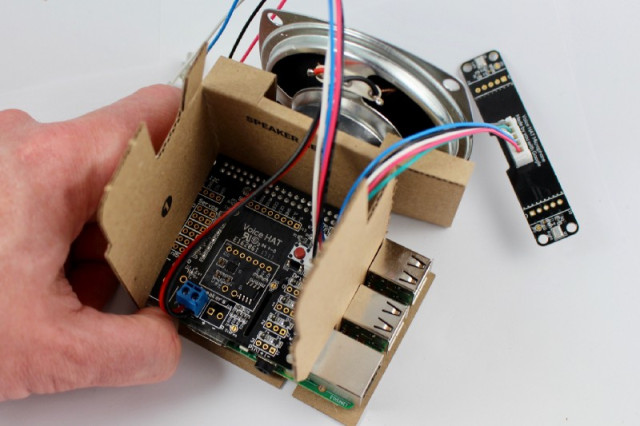
\includegraphics[scale=.3]{voice_kit.jpeg}
\end{center}
\caption{Google AIY Voice Kit Hacking.}
\label{Fig1}
\end{figure}

O 'kit' roda sobre uma variação do SO Linux Debian, adaptado especificamente para este fim e já contendo vários scripts em Python para verificação do correto funcionamento do aparelho, testando os microfones e speeker, além da resposta ao comando de voz.

Além do SO citado, o kit utiliza a API do Google Assistant. O Google Assistant é a fusão do Google de Aprendizado de Máquina, Reconhecimento de Fala e Compreensão de Linguagem. Essencialmente, permite que você tenha uma conversa verbal com o Google e receba respostas por voz. O uso mais conhecido do Assistente no momento está nos dispositivos domésticos do Google, mas também está disponível para determinados telefones Android. Eventualmente, estará disponível em quase toda parte.

\section{\uppercase{Citações e referências}}


\cite{Cunha2018};
\cite{Nazario2017};
\cite{Silva2017};
\cite{Costa2017};
\cite{Ribeiro2017};


\bibliography{Referencias}

%\anex
%\begin{anexosenv}
%\onecolumn
% ---



\end{document} 